\chapter{Related Software}
\label{chap:related_software}

There are plenty of programs and libraries for \gls{graph} visualization with different purposes.
There are D3.js, Neo4j, Graphviz, Tulip, Wolfram Grapher, Pajek, and many more, just to name a few.

In this chapter, however, we will focus on just three software products, each with a very different use case and target user base.

\begin{itemize}

\item The first one is \textbf{Obsidian} which is primarily a note-taking application
but provides a graph view of the notes as an interesting and easy-to-use feature. 

\item The second is \textbf{Gephi}, a software focused on in-depth analysis and visualization of large graphs.

\item And finally there is \textbf{Cytoscape.js}. A JavaScript library for graph visualization in the browser.

\end{itemize}

We chose these in particular because Aphantasia could be viewed as a hybrid of the trio.

We will look into three aspects of these products:
\begin{itemize}
  \item Primary use-case and target user base
  \item User experience
  \item Ability to visualize large graphs
\end{itemize}

As the source of data for testing the large-graph visualization capabilities, we chose the dataset of citations between papers
in the field of high-energy physics \cite{snap_cit_hep} (Later refered to as \gls{cithep_dataset}).
It contains 34 546 nodes, 4 215 78 edges, and temporal data (i.e., dates of publication).

This dataset is suitable for our purposes because:
\begin{itemize}
  \item It is large enough to test the capabilities of both the mentioned software and Aphantasia
  \item It is a real-world dataset with temporal data that is going to play a role in visualizing the contents of Aphantasia
\end{itemize}

\section{Obsidian}

Obsidian \cite{obsidian_website} was a direct inspiration for Aphantasia.
It allows users to create, edit, and, most importantly, interlink markdown file notes in the file system.
One Obsidian project is a system directory called a Vault - a set of markdown notes, user settings, plugins, and other files.
The interlinked notes in a Vault form a directed graph, which can be visualized with just a click of a button.
The graph is animated and provides the ability to replay the history of the Vault from the very first note to the current state.

It is apparent from this description that Obsidian is aimed at a general audience of note-takers 
with maybe a slight bias towards graph/data visualization enthusiasts.
It is available for all the major operating systems and has a large community of users and plenty of extensions available through the
community plugins.

\subsection*{Obsidian graph view}

The graph visualization in obsidian (called graph view) is based on a force-directed layout algorithm.
\footnote{We weren't able to find any specifics about the algorithm used in Obsidian.
However, from the way its graph view behaves, it is safe to assume a variation of an FDL algorithm was used.}
It is easy to use and provides an appealing visual representation of the notes.
The graph is animated and interactive, meaning the user can drag nodes around, zoom in and out, and click on nodes to open the associated note.

It is also customizable to some extent.
The nodes' colors can be set based on different filters, such as path, tags, or text search.
Users can also adjust four sliders - central force, repel force, link force, and link distance.
The graph view is swift for small graphs, but the program needs to spend some time indexing the notes for larger graphs.
(Though this is a one-time operation, the indexes are then saved in the Vault).

In Figure \ref{obr:obsidian_common}, one can see a typical Obsidian graph view depicting a small Vault of one of our projects.

In Figure \ref{obr:obsidian_3000}, we converted a part of the CitHep dataset with only the first 3000 nodes
\footnote{The first as in the order they are stored in the dataset file.}
to markdown notes and visualized them in Obsidian.
It took our machine over 10 minutes to index this graph.
Once indexed, the application ran smoothly.

We were unable to visualize the whole dataset without the program crashing or taking too long to index.
However, we found a few examples of larger datasets rendered in Obsidian online, with one containing 22 000 nodes
\cite{obsidian_reddit_large_graph}.

Obsidian is not very good at clustering nodes with a high degree of connectivity.
To our knowledge, it also does not support automatic node coloring based on clusters, modularity, or other data indicators.
Color must be user-defined based on the content and location of the notes.
CitHep nodes do not contain content apart from id and date, so the nodes in Figure \ref{obr:obsidian_3000} are left default gray.

\begin{figure}[p]\centering
  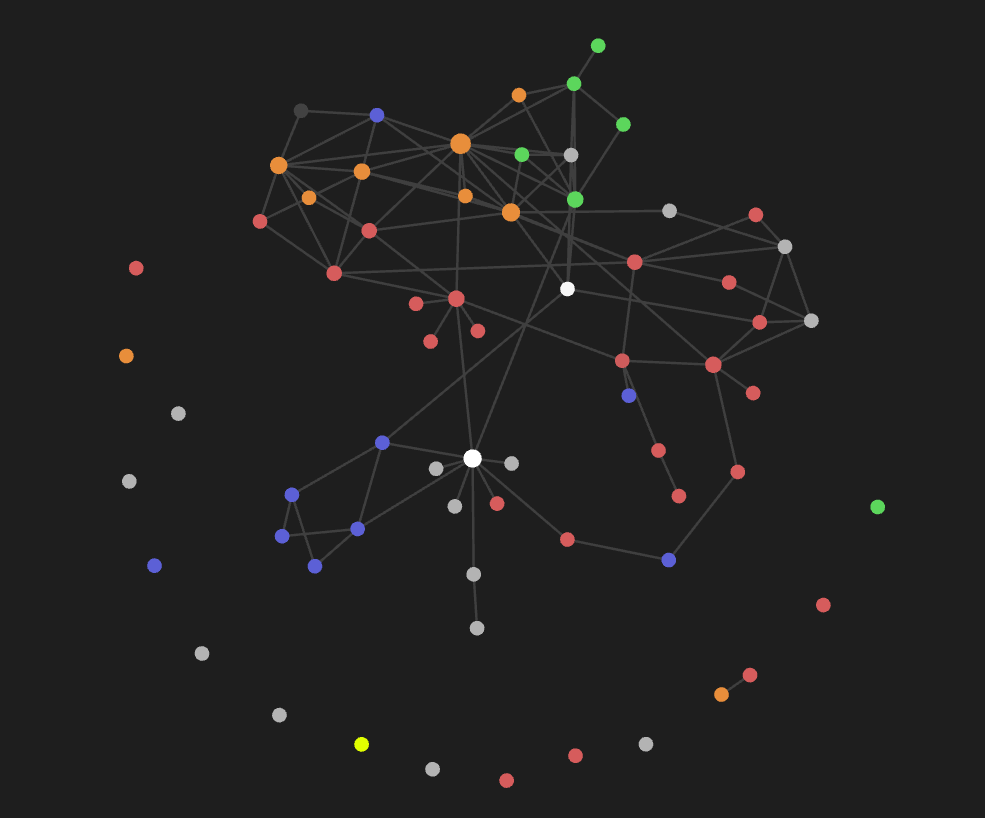
\includegraphics[width=100mm, keepaspectratio]{img/obsidian_common_notes.png}
  \caption{A common graph view of a small Vault in Obsidian}
  \label{obr:obsidian_common}
\end{figure}


\begin{figure}[h]\centering
  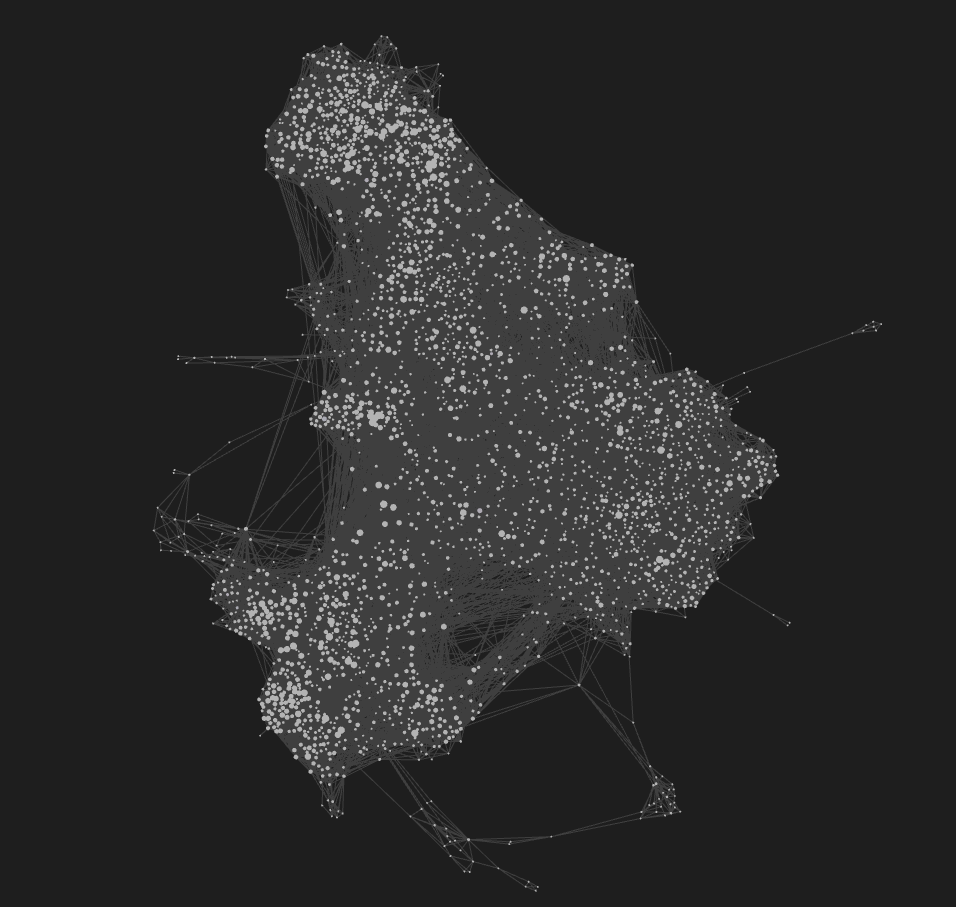
\includegraphics[width=140mm, keepaspectratio]{img/Obsidian_3000}
  \caption{The first 3000 nodes of the CitHep dataset visualized in Obsidian}
  \label{obr:obsidian_3000}
\end{figure}

\section{Gephi}

Much more specialized than Obsidian, Gephi \cite{gephi_homepage} is an open-source software focused on visualization and quantitative analysis of large graphs.
It provides several algorithms for graph layout and quantitative analysis of various data and is extendable through community plugins.

Gephi can compute quantitative characteristics of graph-based data such as modularity, clustering coefficient, degree distribution, and many more.
It can visualize the working data in the viewport and export visually appealing images of the visualized graph.

\subsection*{Gephi graph export}

In Figure \ref{obr:gephi_cithep_3k}, one can see, again, the first 3000 nodes of the CitHep dataset visualized in Gephi.
Compared with Obsidian, the Gephi render export provides more visually identifiable characteristics of the data:

\begin{itemize}
  \item The layout is more structured, and communities are more visible
  \item Colors of the nodes represent their associated modularity class
  \item Size of the nodes represents the number of citations the associated paper has
\end{itemize}

Figure \ref{obr:gephi_cithep} is an exported image of the entire CitHep dataset visualized in Gephi.
The process of exporting this image took a few hours.
We had to learn to use the program itself, import the data,
tweak the layout using various provided algorithms (though we primarily relied on ForceAtlas 2), and finally export the resulting image.

The software crashed a few times during the process, and with the citHep dataset loaded in memory, it wasn't always buttery smooth, but it was otherwise very usable.
Considering the amount of data, that is a commendable feat.

Again, one can find even larger datasets visualized using Gephi.
One post on Gephi forum \cite{gephi_big_graph_forum} shows an exported image of 212 600 nodes and 4 045 203 edges.

The user experience of Gephi is one of a technical tool - something one has to learn to use and spend time with to get the most out of it.
But the reward is the ability to visualize and analyze large graphs better than with any other software we could find.

\begin{figure}[p]\centering
  \includegraphics[width=140mm, keepaspectratio]{img/gephi_first_3000.png}
  \caption{The first 3000 nodes of the CitHep dataset visualized in Gephi}
  \label{obr:gephi_cithep_3k}
\end{figure}


\begin{figure}[p]\centering
  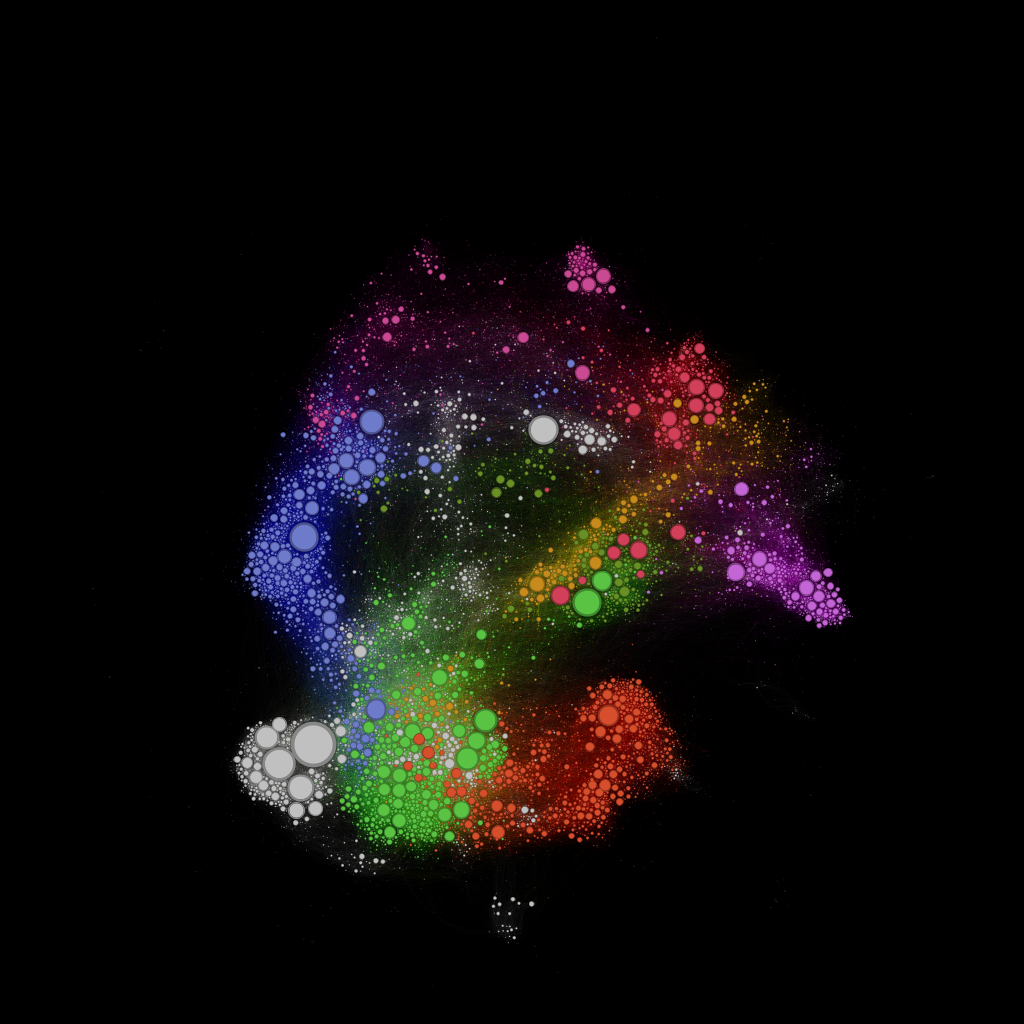
\includegraphics[width=140mm, keepaspectratio]{img/gephi_cithep_35k.png}
  \caption{CitHep dataset visualized in Gephi (34546 nodes)}
  \label{obr:gephi_cithep}
\end{figure}

\section{Cytoscape.js}
\label{sec:cytoscape_js}

Cytoscape.js is a JavaScript library for graph visualization in the browser.
Its homepage starts with a Demos section followed by the headline 'Introduction' and almost 8200 lines of text \cite{cytoscapes_js_homepage}.
Among the demos, there are various examples of usage ranging from simple \glspl{FDL} to more complex use cases such as an interactive graph of wine and cheese pairings.
\cite{wine_and_cheese}

To assess the software, we used two projects - a simple project of our own and one official template showcasing FDL features of the library.

Firstly, we attempted to create a react + cytroscpe.js project.
We initialized a fresh react ts project using \gls{vite}, added the dependency to Cytoscape.js, and, using the official instructions on the Cytoscape.js homepage, we
created a simple application capable of rendering a graph.
See the result in Figure \ref{obr:cytoscape_react_test}.
There is nothing particularly noteworthy about this attempt apart from the fact that the web application uses Cytoscape.js alongside react TypeScript, which seems to be a valid combination of libraries.


\begin{figure}[p]\centering
  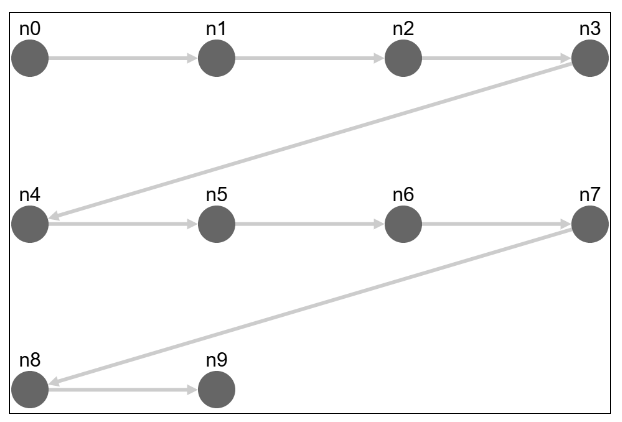
\includegraphics[width=140mm, keepaspectratio]{img/cytoscape_react_10_nodes_path.png}
  \caption{A simple application in react + cytoscape rendering a simple graph}
  \label{obr:cytoscape_react_test}
\end{figure}

The second project was an attempt to render the \gls{cithep_dataset} dataset in Cytoscape.js.
In order to do so, we cloned the GitHub repository of one of the official examples from the cytoscape.js homepage \cite{cytoscapes_js_github}.
The example is called 'Euler' and showcases several small demos using a Cytoscape.js proprietary \gls{FDL}.

The demo called 'Large graph' showcases a path of 5000 nodes and the result can be seen in Figure \ref{obr:cytoscape_5000_nodes_path}.

\begin{figure}[p]\centering
  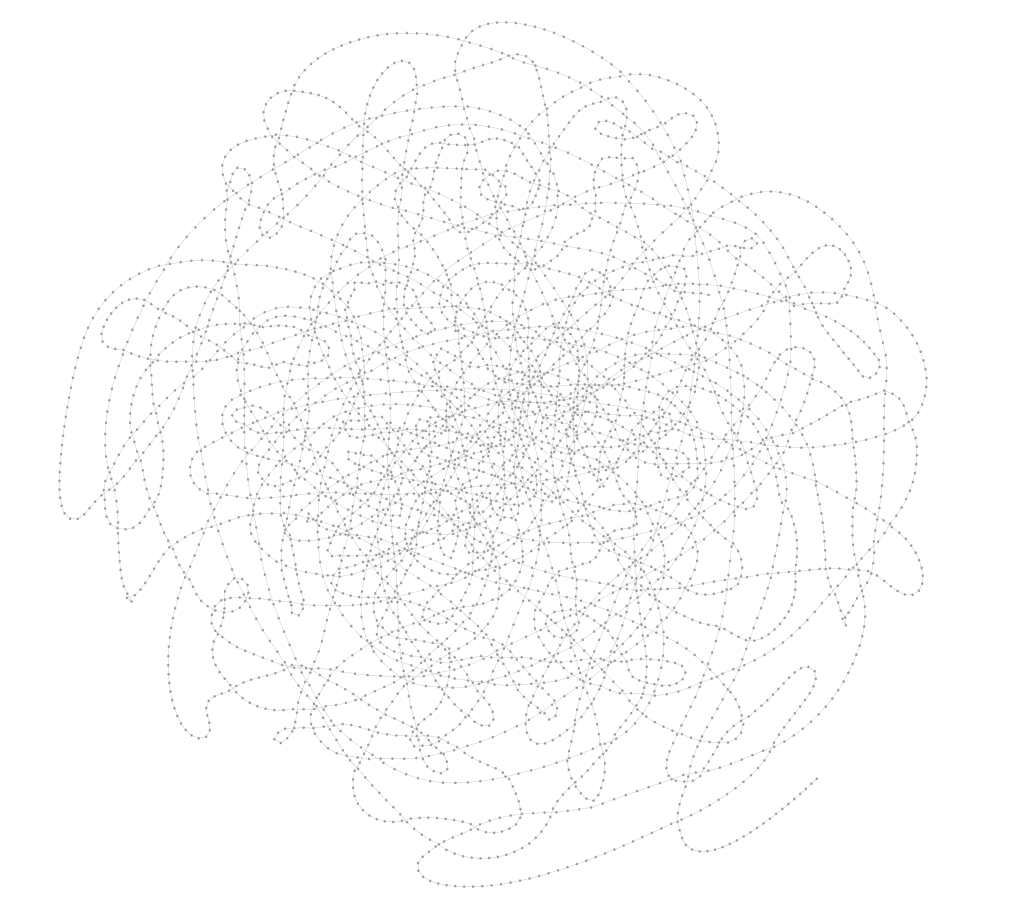
\includegraphics[width=140mm, keepaspectratio]{img/cytoscape_5000_path_official_demo.png}
  \caption{An official example of large graph rendering in Cytoscape.js (path of 5000 nodes)}
  \label{obr:cytoscape_5000_nodes_path}
\end{figure}

This example is animated, and when the page refreshes, the graph stabilizes in real-time.
We had to increase the simulation time as the default value resulted in a tangled, unhelpful layout.
In this case the animation was realtively smooth and with the simulation time set to 10 seconds the graph layout worked well.

We modified this project to use, again, the first 3000 nodes from the CitHep dataset.
We tweaked several parameters such as force strength, edge length, and repulsion strength, and in the end, we achieved the layout shown in Figure \ref{obr:cytoscape_3000_nodes}.
The performance during the runtime of the FDL data dropped under 10 \gls{fps}, but the application remained usable and stable.
The layout we produced was very similar to the one we made with Obsidian.

\begin{figure}[p]\centering
  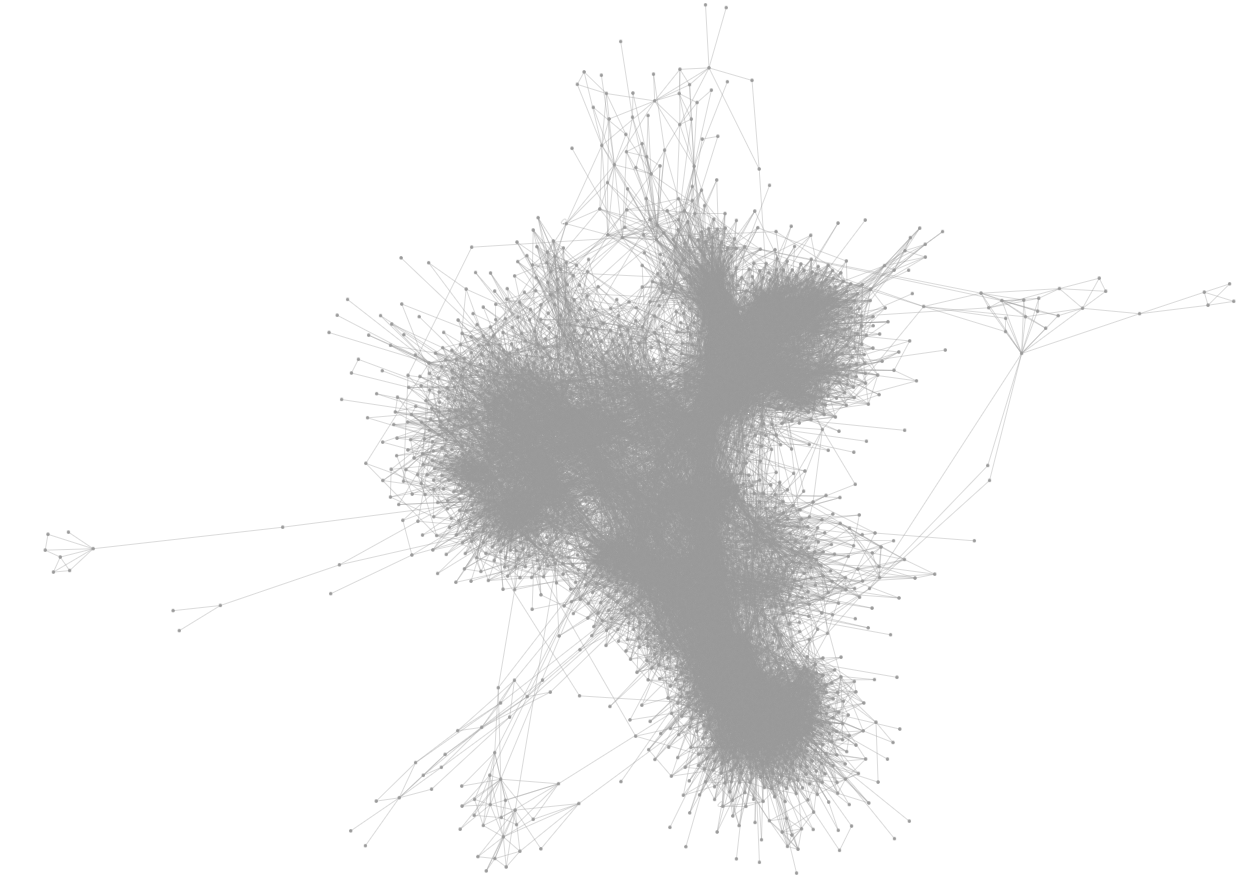
\includegraphics[width=140mm, keepaspectratio]{img/cytoscapejs_cithep_first_3000_nodes.png}
  \caption{The first 3000 nodes of the CitHep dataset visualized in Cytoscape.js}
  \label{obr:cytoscape_3000_nodes}
\end{figure}
We also attempted to render the entire \gls{cithep_dataset} dataset, but unfortunately, the application could not handle it and crashed.

While we did not use the full capabilities of the library, the experience with Cytoscape.js was very positive.
The animations are smooth, there are plenty of parametrization options, and the resulting layout is satisfactory.

\section{Final comparison}
As can be seen in Table \ref{tab:comparison}, the three demonstrated software products vary greatly.
The intended use case and target user base are very different, and so is their large graph rendering capability.

\textbf{Obsidian} is by far the most accessible but offers the least amount of control over the graph layout.

\textbf{Gephi} is the most powerful but also the most complex and time-consuming to use.

\textbf{Cytoscape.js} is a good middle ground between the two but only accessible to developers.

\begin{table}[ht]
  \centering
  \caption{Comparison of Obsidian, Gephi, and Cytoscape.js}
  \label{tab:comparison}
  \begin{tabularx}{\textwidth}{|l|X|X|X|}
    \hline
    \textbf{}                     & \textbf{Obsidian}       & \textbf{Gephi}                      & \textbf{Cytoscape.js} \\ \hline
    \textbf{Use-case}             & note-taking             & data analysis and visualization     & graph visualization in browser \\ \hline
    \textbf{Target Userbase}      & general audience        & researchers,                        & web developers  \\ 
                                  &                         & technical users                     & \\ \hline
    \textbf{User Experience}      & easy to use             & technical,                          & programmatic, \\ 
                                  &                         & steep learning curve                & mostly parametrization\\ \hline
    \textbf{3 000 nodes}           & slow indexing           & stable,                             & stable but  \\ 
    \textbf{handling}             & but smooth afterwards   & smooth                              & visibly lower FPS\\ \hline
    \textbf{34 546 nodes}          & skipped as              & mostly stable,                      & crashed \\
    \textbf{handling}             & indexing took too long  & lower FPS while running FDL         & immediately\\ \hline
  \end{tabularx}
\end{table}